%%%%%%%%%%%%%%%%%%%%%%%%%%%%%%%
%%%%%%%%%%%%%%%%%%%%%%%%%%%%%%%
\chapter{Methods\label{ch:methods}}
%%%%%%%%%%%%%%%%%%%%%%%%%%%%%%%
%Section comments: There were more changes related to objective language and directional words. There is a missing term near line 13.
The system identification of rigid body ship dynamics can be simplified into parameter estimation if parameterized physical models is assumed as the most appropriate model from a collection of candidate models.
The parameter estimations for roll motion and manoeuvring are presented in \autoref{sec:_roll} and \autoref{sec:_VMM}. The most appropriate models are selected in the model development process described in \autoref{sec:cross_validation}.

\section{Roll model parameter estimation} \label{sec:_roll}
\noindent Damping parameters can be estimated directly from the VCT forces, as demonstrated in \autoref{sec:VCT}. However, this approach is not feasible when the ship is free to move, necessitating the use of FT time series data to estimate the parameters. In such cases, the entire dynamics must be considered. The damping parameters ($B_1$, $B_2$, $B_3$) and stiffness parameters ($C_1$, $C_3$, $C_5$) can be identified from the parametric linear, quadratic, and cubic roll motion model structures presented in the previous chapter (\autoref{eq:roll_decay_equation_himeno_linear}, \autoref{eq:roll_decay_equation_himeno_quadratic_b}, and \autoref{eq:roll_decay_equation_cubic}).
These equations do not have unique solutions because each equation can be multiplied by an arbitrary factor to yield a new valid solution. To obtain unique solutions, inertia is excluded by normalizing the equations with the total roll inertia $A_{44}$, as shown in \autoref{eq:roll_decay_nonedim_a44} for the linear model.

\begin{equation} \label{eq:roll_decay_nonedim_a44}
\ddot{\phi} + \frac{B_{1}}{A_{44}} \dot{\phi} + \frac{C_{1}}{A_{44}} \phi = 
\ddot{\phi} + B_{1A} \dot{\phi} + C_{1A} \phi = 0
\end{equation}

\noindent The identified normalized damping and stiffness parameters $B_{1A}$ and $C_{1A}$ can be expressed in dimensional units by multiplication with the normalization factor $A_{44}$. If $A_{44}$ is unknown before hand, it can be calculated using \autoref{eq:A_44_eq} \cite{piehlShipRollDamping2016}, assuming that the meta center height $GM$ is known.
\begin{equation} \label{eq:A_44_eq}
A_{44} = \frac{GM g m}{\omega_{0}^{2}}
\end{equation}

The frequency $\omega_0$ can be obtained with Fast Fourier transform (FFT) of the roll signal. 
Two methods for parameter estimation have been investigated: the \say{derivation approach}, referred to in \textcite{imo1200InterimGuidelines2006}, and the \say{integration approach} used in \textcite{soderAssessmentShipRoll2019} which are both described in the next subsections. 

%\subsection{Inverse dynamics regression}\label{sec:derivation_approach}
In inverse dynamics regression (called derivation approach in Paper \ref{pap:rolldamping}), \autoref{eq:roll_decay_nonedim_a44} is treated as a linear regression problem, where the states ($\phi$, $\dot{\phi}$, $\ddot{\phi}$) are known and the parameters $B_1$ and $C_1$ must be regressed. Only roll angle $\phi$ is known from the experimental data, which means that the velocity and acceleration $\dot{\phi}$, $\ddot{\phi}$ also must be approximated (note that this is done with numerical differentiation in Paper \ref{pap:rolldamping} and with the extended Kalman filter (EKF) in Paper \ref{pap:pit}).
A least squares fit is applied to the roll motion equation to identify the damping and stiffness parameters.

%\subsection{Integration approach}\label{sec:integration_approach}
In the integration approach, \autoref{eq:roll_decay_nonedim_a44} is solved as an ordinary differential equation (ODE) for many estimated sets of parameters until the solution converges. This method is time-consuming, and convergence is not guaranteed. However, the advantage is that only roll angle $\phi$ is needed.
\section{Parameter estimation from virtual captive tests} \label{sec:VCT}
The computational cost of CFD calculations can be significantly reduced by assuming a memory-less state space model (\autoref{eq:state_space}) -- the Markov process assumption \cite{yoonIdentificationHydrodynamicCoefficients2003}. This means that the forces acting on the ship at each time instant can be built up as a series of independent static flow calculations. 
The independence means that the static flow calculations are independent of time, and the order in which they are calculated does no longer matter. The Markov process assumption opens up for a large gain in computational efficiency from the fact that the ship experiences the same state $\mathbf{x}$ and input $\mathbf{u}$ -- or very similar state and input -- several times during a maneuver. This means that the same static flow result can be reused several times -- or at least conceptually, we can think of it that way. Concretely this is achieved by identifying a prediction model to the static flow results, the VCT data, so that forces for each state during the maneuver can be predicted. 
One of the challenges with VCT is to make a good selection of static flow calculations. This means having a VCT matrix that contains the most important states during the maneuver, filling the relevant parts of the state space.  

The ship kinematics are defined by the velocity vector $\pmb{\bm{\upsilon}}$ and the input vector $\mathbf{u}$ so that the forces for each state can be uniquely defined by the velocities $u$, $v$, and $r$, and the input forces from the rudder and propeller. If these forces are then uniquely defined by the thrust and rudder angle, this means that the state space spans at least five dimensions, which would require a lot of VCT calculations to cover the whole state space.
Another challenge with VCT is therefore to select a prediction model -- the manoeuvring model -- that resembles as much of the true hydrodynamics as possible, so that high accuracy can be obtained without having to span the whole state space.  
\autoref{tab:VCT_wPCC} and \autoref{tab:VCT_optiwise} show the VCT matrices for the wPCC and Optiwise test cases.
The coverage of the yaw rate and drift angle space is shown by the phase plots in \autoref{fig:phase_plots}.
% wPCC
\begin{table}[h]
    \centering
    \small
    \caption{State variations with VCT for wPCC.}
    \label{tab:VCT_wPCC}
    \pgfplotstabletypeset[col sep=comma, column type=c, style=string type,
        columns/Test type/.style={column type=l,string type},
        columns/V/.style={column type=c,string type, column name=$V$ [m/s]},
        columns/beta_deg/.style={column type=c,string type, column name=$\beta$ [deg]},
        columns/r/.style={column type=c,string type, column name=$r$ [rad/s]},
        columns/delta_deg/.style={column type=c,string type, column name=$\delta$ [deg]},
        columns/rev/.style={column type=c,string type, column name=rev [1/s]},
        %columns/r/.style={column type=r,fixed,fixed zerofill,precision=2, column name=$r$ [rad/s]},
        %columns/V_R/.style={fixed,fixed zerofill,precision=2, column name=$V_R$ [m/s]},
        %columns/gamma_deg/.style={fixed,fixed zerofill,precision=1, column name=$\gamma$ [deg]},
        %columns/Y_R/.style={fixed,fixed zerofill,precision=1, column name=$Y_R^{VCT}$ [N]},
        %columns/Y_R_MMG/.style={fixed,fixed zerofill,precision=1, column name=$Y_R^{MMG}$ [N]},
        every head row/.style={before row=\hline,after row=\hline},
        every last row/.style={after row=\hline}
    ]{tables/methodology_VCT_wPCC.variations.csv}
\end{table}
% Optiwise
\begin{table}[h]
    \centering
    \small
    \caption{State variations with VCT for Optiwise.}
    \label{tab:VCT_optiwise}
    \pgfplotstabletypeset[col sep=comma, column type=c, style=string type,
        columns/Test type/.style={column type=l,string type},
        columns/V/.style={column type=c,string type, column name=$V$ [m/s]},
        columns/beta_deg/.style={column type=c,string type, column name=$\beta$ [deg]},
        columns/r/.style={column type=c,string type, column name=$r$ [rad/s]},
        columns/delta_deg/.style={column type=c,string type, column name=$\delta$ [deg]},
        columns/rev/.style={column type=c,string type, column name=rev [1/s]},
        %columns/r/.style={column type=r,fixed,fixed zerofill,precision=2, column name=$r$ [rad/s]},
        %columns/V_R/.style={fixed,fixed zerofill,precision=2, column name=$V_R$ [m/s]},
        %columns/gamma_deg/.style={fixed,fixed zerofill,precision=1, column name=$\gamma$ [deg]},
        %columns/Y_R/.style={fixed,fixed zerofill,precision=1, column name=$Y_R^{VCT}$ [N]},
        %columns/Y_R_MMG/.style={fixed,fixed zerofill,precision=1, column name=$Y_R^{MMG}$ [N]},
        every head row/.style={before row=\hline,after row=\hline},
        every last row/.style={after row=\hline}
    ]{tables/methodology_VCT_optiwise.variations.csv}
\end{table}
\begin{figure}[H]
     \centering
     \begin{subfigure}[b]{0.49\textwidth}
         \centering
         \includesvg[width=0.99\textwidth]{figures/methodology_VCT_wPCC.phase_plot.svg}
        \caption{wPCC.}
        \label{fig:VCT_phase_plot_wPCC}
     \end{subfigure}
     \hfill
     \begin{subfigure}[b]{0.49\textwidth}
        \centering
        \includesvg[width=0.99\textwidth]{figures/methodology_VCT_optiwise.phase_plot.svg}
        \caption{Optiwise.}
        \label{fig:VCT_phase_plot_optiwise}
     \end{subfigure}
        \caption{Phase plots of the zigzag tests together with the coverage of the VCTs and extra state VCTs.}
        \label{fig:phase_plots}
\end{figure}

The hydrodynamic damping forces are calculated from the VCT results $X_{VCT}$, $Y_{VCT}$ and $N_{VCT}$
with \autoref{eq:X_D} -- \autoref{eq:N_D}.
\begin{equation}
    \label{eq:X_D}
    X_{D} = X_{VCT} + Y_{\dot{r}} r^{2} + Y_{\dot{v}} r v
\end{equation}
\begin{equation}
    \label{eq:Y_D}
    Y_{D} = - X_{\dot{u}} r u + Y_{VCT}
\end{equation}
\begin{equation}
    \label{eq:N_D}
    N_{D} = N_{VCT} + X_{\dot{u}} u v - Y_{\dot{r}} r u - Y_{\dot{v}} u v
\end{equation}
The mass $m$ has disappeared from \autoref{eq:F_expanded} to arrive at these expressions, because the ship is not moving in ShipFlow -- the CFD tool used in the static flow calculations -- instead the water is having an either oblique or circular inflow \cite{roychoudhuryCFDSimulationsSteady2017}.
The hull forces are calculated by subtracting the contributions of the rudder and propeller from the total forces (\autoref{eq:X_H_VCT} -- \autoref{eq:N_H_VCT}).
\begin{equation}
    \label{eq:X_H_VCT}
    X_H = X_D - X_R - X_P
\end{equation}
\begin{equation}
    \label{eq:Y_H_VCT}
    Y_H = Y_D - Y_R
\end{equation}
\begin{equation}
    \label{eq:N_H_VCT}
    N_H = N_D - N_R
\end{equation}
These forces are used together with the hull force model (\autoref{eq:X_H} -- \autoref{eq:N_H}) to define a linear regression problem that is solved with the ordinary least squares (OLS) method. 
\section{Inverse dynamics} \label{sec:ID}
The forces acting on the ship during a maneuver can be estimated with inverse dynamics from the equation of motion (\autoref{eq:eom}) when the mass matrix $\mathbf{M}$ and the acceleration vector $\pmb{\bm{\dot{\upsilon}}}$ are known. The hydrodynamic damping forces can be calculated by inserting the total force $\mathbf{F}$ from \autoref{eq:F_expanded} into \autoref{eq:eom} and then solve for $X_D$, $Y_D$, and $N_D$ as shown in \autoref{eq:ID_X}-\autoref{eq:ID_N}.
\begin{equation}
    \label{eq:ID_X}
    X_{D} = - X_{\dot{u}} \dot{u} + Y_{\dot{r}} r^{2} + Y_{\dot{v}} r v + \dot{u} m - m r^{2} x_{G} - m r v
\end{equation}
\begin{equation}
    \label{eq:ID_Y}
    Y_{D} = - X_{\dot{u}} r u - Y_{\dot{r}} \dot{r} - Y_{\dot{v}} \dot{v} + \dot{r} m x_{G} + \dot{v} m + m r u
\end{equation}
\begin{equation}
    \label{eq:ID_N}
    N_{D} = I_{z} \dot{r} - N_{\dot{r}} \dot{r} - N_{\dot{v}} \dot{v} + X_{\dot{u}} u v - Y_{\dot{r}} r u - Y_{\dot{v}} u v + \dot{v} m x_{G} + m r u x_{G}
\end{equation}
These expressions are used to estimate the forces acting on the ship during FRMTs, for instance as shown for a turning circle test in \autoref{fig:ID}.
\begin{figure}[H]
    \centering
    \includegraphics[width=\textwidth]{kappa/images/1.pdf}
    \caption{Forces and moments calculated with inverse dynamics on data from a turning circle test.}
    \label{fig:ID}
\end{figure}

The estimated inverse dynamics forces were used in Paper \ref{pap:pit} and \ref{pap:physics} as input to an inverse dynamics regression (see \autoref{sec:IDR}). 

Inverse dynamics was also used in Paper \ref{pap:physics} and \ref{pap:vct} to estimate the forces acting on the ship during the FRMTs to be compared with the model force predictions. This is a more informative way to assess model performance than, for instance, using open-loop or closed-loop simulations. The benefit is that the model and experiment will always be at the same state, which is not the case when simulations are used.
\section{Parameter estimation from inverse dynamics} \label{sec:IDR}
Parameter estimation from CT data (CMT or VCT), as described in \autoref{sec:VCT}, is the classic approach to identifying parameters within a manoeuvring model. However, a model can also be identified from time series FT data obtained with FRMTs or full-scale maneuvers. Rather than, as in the CMT or VCT, directly measuring forces, they can be estimated through the application of inverse dynamics (see \autoref{sec:ID}). However, inverse dynamics is inherently limited in estimating rudder forces, which affects the estimation accuracy of the other manoeuvring coefficients \cite{arakiEstimatingManeuveringCoefficients2012}. It may be difficult to determine where the forces are generated by solely considering the total force, which introduces a high multicollinearity between the hull and the rudder forces during the maneuvers.
This can be addressed by measuring the rudder force, as demonstrated in the Optiwise test case in Paper \ref{pap:vct}. Otherwise, the rudder force must be estimated, which was investigated in Paper \ref{pap:physics} by introducing a semi-empirical rudder model (see \autoref{sec:semi-empirical}). The hull forces needed to regress the hull coefficients can be estimated by subtracting the rudder and propeller forces from the total damping forces according to \autoref{eq:X_H_VCT}--\autoref{eq:N_H_VCT}.




\section{Fourier series method}
\label{sec:fourier}
%\input{kappa/method PIT}
%\subsection{Inverse dynamics regression} \label{sec:IDR}
Finding the hydrodynamic derivatives can be defined as a linear regression problem following the ''derivation approach'' (see \autoref{sec:derivation_approach}):
\begin{equation}\label{equation:03.01_inverse_dynamics:eqregression}
\begin{split}y = X\gamma + \epsilon\end{split}
\end{equation}

\noindent The label vector \(y\) and feature matrix \(X\) in the regression problem in \autoref{equation:03.01_inverse_dynamics:eqregression} can be calculated if model for the hydrodynamic forces is assumed. For example: the label in the regression of the surge degree of freedom for the MAVMM can be calculated using the inverse dynamics force, which is expressed with primed units:
\begin{equation}\label{equation:03.01_inverse_dynamics:diff_eq_X_y}
\begin{split}\displaystyle y = - X_{\dot{u}} \dot{u}' + \dot{u}' m' - m' r'^{2} x_{G'} - m' r' v'\end{split}
\end{equation}

\noindent The feature matrix \(X\) is expressed as:
\begin{equation}\label{equation:03.01_inverse_dynamics:diff_eq_X_X}
\begin{split}\displaystyle X = \left[\begin{matrix}thrust' & u' & \delta^{2} & r'^{2} & u'^{2} & r' v'\end{matrix}\right]\end{split}
\end{equation}

\noindent The hydrodynamic derivatives in the \(\gamma\) vector (\autoref{equation:03.01_inverse_dynamics:diff_eq_X_beta}) can be estimated with ordinary least squares (OLS) regression.
\begin{equation}\label{equation:03.01_inverse_dynamics:diff_eq_X_beta}
\begin{split}\displaystyle \gamma = \left[\begin{matrix}X_{T}\\X_{u}\\X_{\delta\delta}\\X_{rr}\\X_{uu}\\X_{vr}\end{matrix}\right]\end{split}
\end{equation}
In this regression, the hydrodynamic derivatives are treated as Gaussian random variables. The hydrodynamic derivatives in the manoeuvring model are usually estimated as the mean value of each regressed random variable, which is the most likely estimate. The regression result can be expressed with a multivariate Gaussian distribution, which is defined by the regression’s mean values and covariance matrix. The multivariate Gaussian distribution can be used to conduct Monte Carlo simulations in the study of alternative realizations of the regression.

Strong multicollinearity is a documented problem for the manoeuvring models \cite{luo_parameter_2016, wang_quantifying_2018}.
The thrust coefficient \(X_T\) in the hydrodynamic function \(X_D\) in \autoref{equation:02.01_manoeuvring models:eqxabkowitz} introduces multicollinearity to the regression. This coefficient can instead be calculated from the thrust deduction factor \(t_{df}\):
\begin{equation}\label{equation:03.01_inverse_dynamics:eqXthrust}
\begin{split}\displaystyle X_{T} = 1 - t_{df}\end{split}
\end{equation}

\noindent The \(X_T\) coefficient is excluded from the regression by moving it to the left-hand side of the regression equation \autoref{equation:03.01_inverse_dynamics:eqregression}:
\begin{equation}\label{equation:03.01_inverse_dynamics:eqexclude}
\begin{split}y-X_T \cdot thrust = X \gamma + \epsilon\end{split}
\end{equation}

\noindent Rudder coefficients (\(Y_R\)) from \(Y_D\) equation \autoref{equation:02.01_manoeuvring models:eqyabkowitz}, such as \(Y_{\delta}\) and \(Y_{\delta T}\), have also been excluded by assuming a connection with their \(N_D\) equation counterpart through the rudder lever arm \(x_r\):
\begin{equation}\label{equation:03.01_inverse_dynamics:eqyr}
\begin{split}\displaystyle Y_{R} = \frac{N_{R}}{x_{r'}}\end{split}
\end{equation}

\subsection{Inverse dynamics and regression}
\label{\detokenize{03.01_inverse_dynamics:inverse-dynamics-and-regression}}\label{\detokenize{03.01_inverse_dynamics::doc}}

Each manoeuvring model has some hydrodynamic functions \(X_D(u,v,r,\delta,thrust)\), \(Y_D(u,v,r,\delta,thrust)\), \(N_D(u,v,r,\delta,thrust)\) that are defined as polynomials. The hydrodynamic derivatives in these polynomials can be identified with force regression of measured forces and moments. The measured forces and moments are usually taken from captive model tests (CMT), planar motion mechanism (PMM) tests, or virtual captive tests (VCT). However, motions are recorded when the ship is free in all degrees of freedom. Hence, forces and moments causing ship motion must be estimated by solving the inverse dynamics problem.
The inverse dynamics problem is solved by restructuring the system equation (\autoref{equation:02.01_manoeuvring models:eqacc}) to get the hydrodynamics functions on the left-hand side. If the mass and inertia of the ship with added masses: \(X_{\dot{u}}\), \(Y_{\dot{v}}\), \(Y_{\dot{r}}\), \(N_{\dot{v}}\), and \(N_{\dot{r}}\) are known; the forces in the Prime system can be calculated using \autoref{equation:03.01_inverse_dynamics:eqxd}, \autoref{equation:03.01_inverse_dynamics:eqyd}, and \autoref{equation:03.01_inverse_dynamics:eqnd}.
These forces can be used to regress the hydrodynamic derivatives through the ordinary least square (OLS) method. If the added masses are unknown, they can be calculated using potential flow methods or semi-empirical methods (\autoref{app:initial_estimates}). 
\begin{equation}\label{equation:03.01_inverse_dynamics:eqxd}
\begin{split}\displaystyle \operatorname{X_{D}'}{\left(u',v',r',\delta,thrust' \right)} = - X_{\dot{u}}' \dot{u}' + \dot{u}' m' - m' r'^{2} x_{G}' - m' r' v'\end{split}
\end{equation}\begin{equation}\label{equation:03.01_inverse_dynamics:eqyd}
\begin{split}\displaystyle \operatorname{Y_{D}'}{\left(u',v',r',\delta,thrust' \right)} = - Y_{\dot{r}}' \dot{r}' - Y_{\dot{v}}' \dot{v}' + \dot{r}' m' x_{G}' + \dot{v}' m' + m' r' u'\end{split}
\end{equation}\begin{equation}\label{equation:03.01_inverse_dynamics:eqnd}
\begin{split}\displaystyle \operatorname{N_{D}'}{\left(u',v',r',\delta,thrust' \right)} = I_{z}' \dot{r}' - N_{\dot{r}}' \dot{r}' - N_{\dot{v}}' \dot{v}' + \dot{v}' m' x_{G}' + m' r' u' x_{G}'\end{split}
\end{equation}

An example that includes forces calculated with inverse dynamics from motions in a turning circle test can be seen in \hyperref[\detokenize{03.01_inverse_dynamics:fig-inverse}]{\autoref{\detokenize{03.01_inverse_dynamics:fig-inverse}}}. The forces have been converted to SI units.

\begin{figure}[H]
    \centering
    \includegraphics[width=\textwidth]{kappa/images/1.pdf}
    \caption{Forces and moments calculated with inverse dynamics on data from a turning circle test.}
    \label{\detokenize{03.01_inverse_dynamics:fig-inverse}}
\end{figure}
\section{Data cleaning}
\label{sec:datacleaning}
It is possible to perform an exact parameter estimation on flawless (simulated) data with no noise (see Paper \ref{pap:pit}). However, such ideal data from physical experiments do not exist in reality. Measured data will always contain both process noise and measurement noise. Even very moderate measurement noise can create significant problems for inverse dynamics in cases where noise is amplified when velocities and accelerations are differentiated from measured positions.
Mitigation of the effects of noise can be achieved if the data are pre-processed using the extended Kalman filter (EKF) \cite{brownIntroductionRandomSignals1997} and the Rauch-Tung-Striebel (RTS) smoother \cite{rauchMaximumLikelihoodEstimates1965}, both of which are presented below.

EKF is an extension of the Kalman filter (KF) that is used for nonlinear systems, such as manoeuvring models. The premise is that noise can be neglected in the absence of a plausible physical explanation. For instance, if noisy measurement data were entirely correct,it would imply that large ship vibrations resulted from large high-frequency forces (given the size of the ship). A prior understanding of the system dynamics suggests that these forces are not present. Therefore, the noise should be considered measurement noise and should be removed. Low-pass filtering is commonly used to remove noise, where motions above a cutoff frequency are considered unphysical measurement noise. However, choosing this cutoff frequency is difficult. It is often  either too low (removing some of the signal) or too high (retaining some unfiltered measurement noise in the data). The Kalman filter has a predictor model, a manoeuvring model in this case, that continuously estimates the system’s state that runs parallel with the measurement data. The filter estimates the current state as a combination of the measurement data and the predictor model estimate based on the possible validity of the data and the model. If the data has low noise, the estimate is closer to that data. Conversely, if the model provides very accurate predictions, then that estimate is closer to the model.
The system’s inverse dynamics require everything about the state (positions, velocities, and accelerations) to be known. Only positions are known from the measurements, so the velocities and accelerations are instead estimated by the EKF.

The EKF is recursive and updates estimates in real-time as new measurements become available. It uses past measurements to predict states in the near future, making it useful for online applications, such as autopilots or autonomous ships. However, this real-time constraint is unnecessary for the estimation of pre-existing data, where an entire time series of existing measurements is available. In such cases, knowledge of both past and future data can be used to improve the filter. Future time steps can be included by applying the RTS smoother after the filter. The RTS smoother algorithm runs the EKF in reverse to account for future time steps. The EKF recursive algorithm used is summarized in the pseudo-code in \autoref{fig:ek-algorithm} \cite{brownIntroductionRandomSignals1997}.
\clearpage
\label{04.01_EK:ek-algorithm}
\begin{sphinxadmonition}{note}{Algorithm 3.1 (Discrete\sphinxhyphen{}time extended Kalman filter)}



\sphinxAtStartPar
\sphinxstylestrong{Inputs} Initial values: \(x_0\), \(P_0\), \(C_d\), \(R_d\), \(Q_d\), \(E_d\)

\sphinxAtStartPar
\sphinxstylestrong{Output} Estimated states: \(\hat{x}\), estimated state covariances \(\hat{P}\)
\begin{enumerate}
\sphinxsetlistlabels{\arabic}{enumi}{enumii}{}{.}%
\item {} 
\sphinxAtStartPar
Initial values:
\begin{enumerate}
\sphinxsetlistlabels{\arabic}{enumii}{enumiii}{}{.}%
\item {} 
\sphinxAtStartPar
\(\hat{x}[0] = x_0\)

\item {} 
\sphinxAtStartPar
\(\hat{P}[0] = P_0\)

\end{enumerate}

\item {} 
\sphinxAtStartPar
For \(k\) in \(n\) measurements (time steps)
\begin{enumerate}
\sphinxsetlistlabels{\arabic}{enumii}{enumiii}{}{.}%
\item {} 
\sphinxAtStartPar
KF gain
\begin{enumerate}
\sphinxsetlistlabels{\arabic}{enumiii}{enumiv}{}{.}%
\item {} 
\sphinxAtStartPar
\(K[k]=\hat{P}[k] C_d^T \left(C_d \hat{P}[k] C_d^T + R_d\right)^{-1}\)

\item {} 
\sphinxAtStartPar
\(I_{KC} = I_n - K[k] C_d\)

\end{enumerate}

\item {} 
\sphinxAtStartPar
Update
\begin{enumerate}
\sphinxsetlistlabels{\arabic}{enumiii}{enumiv}{}{.}%
\item {} 
\sphinxAtStartPar
State corrector
\(\hat{x}[k] = \hat{x}[k] + K[k] (y - C_d \hat{x}[k]) \)

\item {} 
\sphinxAtStartPar
Covariance corrector
\(\hat{P}[k] = I_{KC} \cdot \hat{P}[k] I_{KC}^T + K[k] R_d K^T \)

\end{enumerate}

\item {} 
\sphinxAtStartPar
Predict
\begin{enumerate}
\sphinxsetlistlabels{\arabic}{enumiii}{enumiv}{}{.}%
\item {} 
\sphinxAtStartPar
State predictor
\(\hat{x}[k+1] = \hat{x}[k] + h \cdot \hat{f}(\hat{x}[k], c[k])\)

\item {} 
\sphinxAtStartPar
Covariance predictor
\(\hat{P}[k+1] = A_d[k]  \hat{P}[k] A_d[k]^T + E_d Q_d E_d^T \)

\end{enumerate}

\end{enumerate}

\end{enumerate}
\end{sphinxadmonition}
Here, \(n\) is the number of states (6 in this case), and \(\mathbf{I_n}\) is an $n$ by $n$ identity matrix.
The transition matrix is calculated for each iteration using the Jacobian of the transition model:
\begin{equation}\label{equation:04.01_EK:eqjacobi}
\begin{split}\mathbf{A_d}[k] = \mathbf{I_n} + h \left. \frac{\partial f \left(\mathbf{x}[k],\mathbf{c}[k] \right)}{\partial \mathbf{x}[k]} \right|_{\mathbf{x}[k]=\mathbf{\hat{x}}[k]}\end{split}
\end{equation}
This formulation and the fact that the nonlinear transition model is used directly as the predictor are the key differences between the EKF and the linear KF. Please note the linear approximation in \autoref{equation:04.01_EK:eqjacobi} around the current state. This approximation can cause instability if the real system and the linearized system deviate significantly when large time steps are used on a very nonlinear system. The unscented Kalman filter, which was used in \textcite{revestidoherreroTwostepIdentificationNonlinear2012}, is an alternative that can be applied in such situations.

The output from the filter contains the estimated states: \(\mathbf{\hat{x}}\) and the estimated state covariance matrix \(\mathbf{\hat{P}}\). \(\mathbf{\hat{x}}\) represents the most likely estimates, but these estimates have uncertainty that is expressed in \(\mathbf{\hat{P}}\).
The state of the system is described by the ship's position, heading, velocities, and yaw velocity:
\begin{equation}\label{equation:04.01_EK:eqstates}
\begin{split}\mathbf{x} = [x_0,y_0,\psi,u,v,r]^T\end{split}
\end{equation}

The initial state \(x_0\) is taken as the mean value of the first five measurements, where the velocities are estimated using numeric differentiation.
\(\mathbf{C_d}\) selects the measured states (\(x_0\), \(y_0\), \(\psi\)):
\begin{equation}\label{equation:04.01_EK:eqcd}
\begin{split}\displaystyle \mathbf{C_{d}} = h \left[\begin{matrix}1 & 0 & 0 & 0 & 0 & 0\\0 & 1 & 0 & 0 & 0 & 0\\0 & 0 & 1 & 0 & 0 & 0\end{matrix}\right]\end{split}
\end{equation}
\(\mathbf{E_d}\) selects the hidden states (\(u\), \(v\), \(r\)):
\begin{equation}\label{equation:04.01_EK:eqed}
\begin{split}\displaystyle \mathbf{E_{d}} = h \left[\begin{matrix}0 & 0 & 0\\0 & 0 & 0\\0 & 0 & 0\\1 & 0 & 0\\0 & 1 & 0\\0 & 0 & 1\end{matrix}\right]\end{split}
\end{equation}
where \(h\) is the discrete time step, \(\mathbf{R_d}\) describes the covariance matrix of the measurement, \(\mathbf{Q_d}\) is the covariance matrix of the process model, and \(\mathbf{P_0}\) is the initial state covariance.
Selecting appropriate values for these three matrices is the most challenging aspect of optimizing EKF performance. The matrix \(\mathbf{R_d}\) should reflect the expected measurement noise,  and  \(\mathbf{Q_d}\) should account for the uncertainty introduced by the process model (manoeuvring model) .
\section{Recursive inverse dynamics regression} \label{sec:_VMM}
A new parameter estimation method is proposed in Paper \ref{pap:pit} for the manoeuvring model structures. A manoeuvring model is used to solve the reversed manoeuvring problem. The problem may consist of predicting unknown forces from known manoeuvring model test data. The hydrodynamic derivatives in the manoeuvring model can be identified through regression of the force polynomials on forces predicted with inverse dynamics (see \autoref{sec:ID}).
The measurement noise must be removed prior to the regression of hydrodynamic derivatives in the manoeuvring model. This is conducted by an extended Kalman filter (EKF) and a Rauch Tung Striebel (RTS) smoother (see \autoref{sec:datacleaning}). The EKF requires an accurate manoeuvring model as the predictor.
Therefore, the accurate manoeuvring model is both the input and output of the method. As a solution to this dilemma, a linear manoeuvring model that includes hydrodynamic derivatives estimated with semi-empirical formulas (\autoref{app:initial_estimates}) is used as the initial predictor. Once the regressed manoeuvring model has been obtained, the parameter estimation can be refined, using the regressed manoeuvring model as the predictor model in the EKF, to improve the filter and obtain a more accurate manoeuvring model. The method is summarized in \autoref{fig:greyvmm} and can be repeated several times (indicated by the dashed arrow) for improved accuracy. 
\begin{figure}[h]
    
    \centering
    \begin{tikzpicture}[node distance=1.5cm]
    %\draw (0,0) rectangle (10,10); %create a bounding box to reserve space
    \node (data) [io] {\footnotesize Model test data: $x$, $\delta$, thrust};
    
    \node (EKF) [process, right of=data, xshift=3.0cm] {\footnotesize EFK + RTS};
    \node (predictor) [process, right of=EKF, xshift=1.5cm]{\footnotesize Predictor};
    \node (VMM) [io, right of=predictor, xshift=1.0cm] {\footnotesize initial model};
    
    \node (data_clean) [io, below of=EKF] {\footnotesize \(x,\dot{x},\ddot{x}, \delta, thrust\)};
    
    \node (black-box) [black-box, below of=data_clean] {\footnotesize Regression};
    
    \node (X_D) [io, left of=black-box, xshift=-0.70cm, yshift=0.7cm]{\footnotesize \(X_D\)};
    \node (Y_D) [io, left of=black-box, xshift=-0.70cm, yshift=0cm]{\footnotesize \(Y_D\)};
    \node (N_D) [io, left of=black-box, xshift=-0.70cm, yshift=-0.7cm]{\footnotesize \(N_D\)};
    
    \node (white-box) [white-box, left of=Y_D, xshift=-1.00cm] {\footnotesize Inverse dynamics};
    
    
    %
    %
    \node (coefficients) [io, right of=black-box, xshift=1.5cm] {\footnotesize model$\left(Y_{uv},N_{\delta},...\right)$};
    
    \draw [arrow] (data) -- (EKF);
    \draw [arrow] (predictor) -- (EKF);
    \draw [arrow] (VMM) -- (predictor);
    \draw [arrow] (EKF) -- (data_clean);
    
    \draw [arrow] (data_clean) -| (white-box);
    \draw [arrow] (data_clean) -- (black-box);
    
    \draw [arrow] (white-box) -- (X_D);
    \draw [arrow] (white-box) -- (Y_D);
    \draw [arrow] (white-box) -- (N_D);
    
    \draw [arrow, shorten >=0.5cm] (X_D) -- (black-box);
    \draw [arrow, shorten >=0.2cm] (Y_D)  -- (black-box);
    \draw [arrow, shorten >=0.5cm] (N_D)  -- (black-box);
    
    
    \draw [arrow] (black-box)  -- (coefficients);
    \draw [arrow, dashed] (coefficients)  -- (predictor);
    
    \end{tikzpicture}
    \caption{Method to estimate the manoeuvring model hydrodynamic derivatives.}
    \label{fig:greyvmm}
\end{figure}

\noindent Using semi-empirical formulas (\autoref{app:initial_estimates}) for the initially estimated manoeuvring model adds prior knowledge about the ship dynamics to the regression. An example, with simulation results from the steps in the iteration, is presented in \hyperref[\detokenize{01.01_method:iterations}]{\autoref{\detokenize{01.01_method:iterations}}}.


\begin{figure}[H]
    \centering
    \includegraphics[width=\textwidth]{kappa/images/0.pdf}
    \caption{Simulation with: initial model and first and second iteration of the parameter estimation method.}
    \label{\detokenize{01.01_method:iterations}}
\end{figure}
\section{Generalization of models} \label{sec:generalization}
Generalization refers to a model's ability to perform well on new, unseen data, rather than just the data it was trained on. This is crucial because the ultimate goal of a model is to make accurate predictions on real-world data, not just the training dataset. For data driven models overfitting can be a problem. The model learns the training data too well, including noise and outliers so that it performs poorly on new data. The opposite, underfitting the data can also be a problem. The model is too simple to capture the underlying patterns in the data, leading to poor performance on both training and new data.  

The bias–variance tradeoff is a fundamental concept in understanding generalization. A model with high bias (underfitting) makes strong assumptions about the data, while a model with high variance (overfitting) is too sensitive to the training data. The goal is to find a balance between bias and variance to achieve good generalization. Cross validation is one way to prevent overfitting, which is further explained in the next section.

\section{Cross validation}
\label{sec:cross_validation}
The aim of developing a manoeuvring model with parameter estimation is to develop a model that can generalize outside the known data. The method presented in this thesis is assessed with the hold-out evaluation \cite{sammutHoldoutEvaluation2017}. The data in this evaluation is divided into three sets: the training set, the validation set, and the test set as seen in \autoref{fig:model_development_process}.

\begin{figure}[H]
\centering
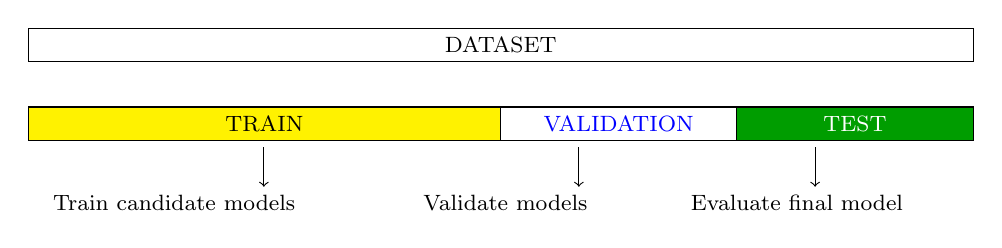
\begin{tikzpicture}

\node (dataset)[rectangle,
    anchor=west,
    draw,
    text = black,
    minimum width=12cm,
    fill = white] at (0, 0) {\footnotesize DATASET};

\node (train)[rectangle,
    draw,
    anchor=west,
    text = black,
    minimum width=6cm,
    fill = yellow] at (0, -1cm) {\footnotesize TRAIN};

\node (validation)[rectangle,
    draw,
    anchor=west,
    text = blue,
    minimum width=3cm,
    fill = white] at (6cm, -1cm) {\footnotesize VALIDATION};

\node (test)[rectangle,
    draw,
    anchor=west,
    text = white,
    minimum width=3cm,
    fill = black!15!green!255] at (9cm, -1cm){\footnotesize TEST};
    
\node (train_multiple)[rectangle,
    draw,
    anchor=west,
    text = black,
    draw = none,
    fill = none] at (0.2cm, -2cm){\footnotesize Train candidate models};
    
\node (validate_models)[rectangle,
    draw,
    anchor=west,
    text = black,
    draw = none,
    fill = none] at (4.9cm, -2cm){\footnotesize Validate models};
    
\node (evaluate_models)[rectangle,
    draw,
    anchor=west,
    text = black,
    draw = none,
    fill = none] at (8.3cm, -2cm) {\footnotesize Evaluate final model};

\draw[->] (3,-1.3) -- (3,-1.8);
\draw[->] (7,-1.3) -- (7,-1.8);
\draw[->] (10,-1.3) -- (10,-1.8);



\end{tikzpicture}
\caption{Model development process with hold-out evaluation.}
\label{fig:model_development_process}
\end{figure}

\noindent The purpose of the training set is to train all the candidate models using the proposed parameter estimation method. The validation set is used to select the most effective candidate model. The training and validation sets are joined to train the selected model as the final model. The final model is used for predicting the test set, which is used to evaluate the accuracy of the model. These three sets are not divided randomly;  they are divided to assess the model’s extrapolation ability. The data sets are therefore split to have the smallest yaw rates, drift-angles, and rudder-angles in the training set; the medium values in the validation set; and the largest values in the test set.
Examples of this can be seen for the two test cases in this thesis in \autoref{fig:kvlcc2_datasets} and  \autoref{fig:wpcc_datasets} in the next chapter.
\section{Test cases} \label{sec:test_cases}
Two test cases have been studied in this thesis. The wPCC test case is a ship that was designed for a wind-assisted propulsion system (WAPS) and is capable of operating in a fully sailing mode, a fully motoring mode, and intermediate states. 
However, this thesis only considers the motoring mode. The wPCC design differs slightly from conventional motoring cargo ship designs because of the WAPS. It has two very large rudders, which are two to three times larger than those needed for a conventional ship. The ship also has fins at the bilge to generate extra lift while sailing, as shown on the scale model in \autoref{fig:wPCC}.
\autoref{tab:main_particulars} shows the main particulars of the scale model. 
\begin{figure}[h]
    \centering
    \includegraphics[width=\columnwidth]{figures/5m2.jpg}
    \caption{Scale model of the wPCC used in the model tests. Copyright RISE.}
    \label{fig:wPCC}
\end{figure}

The Optiwse test case is based on a typical VLCC tanker but features a larger rudder size adapted for the WAPS, as shown in the scale model in \autoref{fig:optiwise}. \autoref{tab:main_particulars} shows the main particulars of the scale model. 
\begin{figure}[h]
    \centering
    \includegraphics[width=\columnwidth]{figures/optiwise.jpg}
    \caption{Scale model of the Optiwise used in the model tests. Copyright RISE.}
    \label{fig:optiwise}
\end{figure}
\begin{table}[h]
    \centering
    \caption{Main particulars of the test case scale models.}
    \label{tab:main_particulars}
    \pgfplotstabletypeset[col sep=comma, column type=r, columns={Parameter,Unit, wPCC, Optiwise, Description},
        columns/Parameter/.style={column type=l,string type},
        columns/Unit/.style={column type=l,string type, column name=~},
        columns/wPCC/.style={column type=r},
        columns/Optiwise/.style={column type=r},
        columns/Description/.style={column type=l,string type},
        every head row/.style={before row=\hline,after row=\hline},
        every last row/.style={after row=\hline}
    ]{tables/test_cases.main_particulars.csv}
\end{table}

